\chapter{Stages of Speaker Diarization}
This chapter discusses the general stages of a speaker diarization system and some of the new techniques that are commonly used these days. A good overview of the diarization field, although not up to date, can be found in \cite{anguera2012speaker} and \cite{1677976}. In all diarization systems, the basic approach is to first extract the segments containing speech from the audio, further divide the segments into subsegments in which the speaker identities are constant, represent each subsegment using a speaker embedding, and cluster the subsegments together so that each cluster represents a unique speaker.

\section{Speech Enhancement}
Any speech system needs to address the problem of environmental noise in audio recordings. It is important to remove as much noise as possible, but also speaker information loss should be kept to a minimum. If done right, this stage results in increased performance in subsequent stages. If not, artefacts in denoised speech reduce diarization performance. In recent years, deep learning methods have partially solved the problem of artefacts, but generalization ability in varied domains is still a problem. This stage is not mandatory, but can be helpful in certain conditions.

\section{Feature Extraction}
The first important step in any speech system is to represent the speech recording using a sequence of feature vectors. This representation is much more compact as it only uses a few thousand parameters for every second of audio, compared to 44,100 samples in a raw waveform sampled at 44.1 KHz. The most commonly used features are Mel Frequency Cepstral Coefficients (MFCCs) \cite{logan2000mel}. A brief overview of MFCCs is as follows.

\begin{figure}[h]
	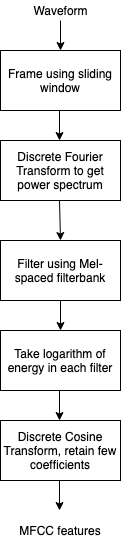
\includegraphics[width=3cm]{figures/mfcc.png}
	\centering
	\caption{Stages of MFCC computation.}
	\label{fig:fig-mfcc}
\end{figure}

Speech production can be thought of as filtering of the sound produced from the vocal cords by the shape of the human vocal tract. The shape is influenced by the positions of the tongue, teeth, lips, velum etc and determines what sound comes out. Since the shape of the vocal tract is manifested in the envelope of the short time power spectrum of the speech signal, the job of the MFCCs can be thought of as to represent this envelope accurately.

As a first step, overlapping frames are extracted from the digitized signal using a sliding window. The properties of the signal are assumed to be stationary in this small window duration. Discrete Fourier Transform (DFT) is applied on each frame to get the periodogram of the frame. This tells us which frequencies are present in the frame. We need this because the cochlea in the human ear vibrates at different spots depending on the frequency composition of the sounds.

This still has too much information and we need to get rid of unnecessary information. The properties of the cochlea can be exploited for this. The cochlea cannot discern the difference between closely spaced frequencies, and this effect gets stronger as the frequencies increase. So to simulate this we can take energies from bins placed on the periodogram at increasing distances. The placement of the bins can be computed by using the Mel Scale \cite{logan2000mel}, which is a perceptual scale of pitches judged by listeners to be equal in distance from one another. It is a logarithmic scale given by the below formula, which models the perceptual behaviour of the cochlea. It converts $f$ Hz to $m$ Mels. The bins are placed equidistant in Mel-domain, so that they are at an increasing distance in Hz-domain. The output of this operation can be interpreted as filtering the periodogram using a triangular filterbank called Mel-filterbank.

$$ m = 2595 \log \left( 1+\frac{f}{700} \right) $$

After filtering and summing the values in say 26 bins, we get 26 energies. Logarithm is applied to each number because loudness is not perceived on a linear scale. Finally, Discrete Fourier Transform (DCT) is applied to these energies which decorrelates the energies, which allows modelling the features using diagonal covariance matrices. The first 12-13 coefficients are kept, rest are discarded. This is the MFCC feature vector for this frame. In cases decorrelated features are not necessary, for example neural networks, the DCT step is avoided and the features are called Mel-Filterbank features or FBANK features.

In most cases the MFCCs are also appended with delta and delta-delta coefficients, which are basically the first and second order derivatives calculated from the original coefficients using a sliding window context. These capture the acceleration trends in the coefficients on top of just their absolute values, and generally increase performance of speech systems.

\section{Speech Activity Detection}
Speech activity detection (SAD) extracts the segments in the audio that contain speech, and discards the rest. This is important because speaker diarization is only concerned with assigning speaker identities to speech segments, and does not need to do anything with non-speech segments. It is also possible to consider all the non-speech segments to be coming from a hypothetical new speaker which gets its own cluster after clustering, but that does not result in good performance as the amount of variability possible in non-speech sounds is too high. Therefore, doing a separate SAD step before diarization is the standard method.

There are two goals of a good SAD system - keep missed speech to a minimum, and keep false alarm speech to a minimum. The first might cause too few speakers to be detected, while the second pollutes clusters and degrades the diarization output. If the diarization system is used as a frontend for ASR, these errors cause word deletion and word insertion errors respectively.

Since this is a binary classification problem, it can be solved by using simple thresholding on the frame energy level. The MFCC features have the log energy of the frame as the first coefficient which can be used for this. Statistical model-based approaches are much more popular and are trained with large amounts of of diverse external data. Typically Long Short Term Memory networks (LSTMs) or Time Delay Neural Networks (TDNNs) are used for this task.

\section{Segmentation}

The goal of the segmentation task is to further divide the speech segments found after the SAD step into smaller subsegments such that there are no speaker turns within any of these subsegments. Speaker turns are defined to be the points in the audio where the set of talking speakers changes. For example within a speech segment, the point where spkr1 changes into spkr2 (spkr1 finished talking and spkr2 started immediately) would be a speaker turn because the set of talking speakers changes from [spkr1] to [spkr2]. Similarly, if spkr2 starts talking without waiting for spkr1 to end (causing an overlap) the set changes from [spkr1] to [spkr1,spkr2], which is also a speaker turn.

There are basically two ways to do segmentation. The first way is to try and automatically detect speaker turns and divide the segments at these points. The classical approach for doing this uses a sliding window, and compares consecutive windows.	The comparison decides whether the two windows are better accounted by two separate models (different speaker sets) or single model (same speaker set) using an empirically determined threshold. Many distance metrics exist for this decision, for example the Delta Bayesian Information Criterion ($\Delta$BIC) \cite{Chen1998SpeakerE} metric. The second way is to divide the segments uniformly into very small subsegments (1-2 seconds) so that it is unlikely that the set of speakers changes within that segment, and assume that it is constant. It is not clear which of these ways yields better results. Uniform segmentation approaches are reported to work better for x-vectors, which are state-of-the-art \cite{patino2018odessa}.

\section{Clustering}
	As the most important step of the diarization process, clustering works on the whole audio recording and groups together segments that belong to the same speaker. In the ideal case, all the segments belonging to a speaker exist in the same cluster, and the number of clusters is equal to the actual number of speakers. The clustering process needs a distance-like similarity measure between pairs of segments to work. Each segment can be represented by a point in vector space or a statistical model. This acts as the speaker representation for the segment, where the distance between any two representations is lower if the segments have speech from the same speaker.
	
	Since the speaker verification and identification fields also use speaker models to capture speaker information, these models are adopted for clustering for diarization. The some of the best performing models are outlined below.
	
	\subsection{Speaker Representation}
		\subsubsection{Gaussian Mixture Models}
		Gaussian Mixture Models (GMMs) are generative models that can be used for modelling multivariate data. In GMMs, the probability of a data point is given by the weighted combination of the probabilities from several multivariate Gaussian distributions having their own mean and covariance matrices.
		
		The goal is to train a GMM to represent each segment. For this, the feature vectors belonging to a segment can simply be pooled together and a GMM can be learned using the Expectation-Maximization (EM) \cite{moon1996expectation} algorithm. But this is a problem because the number of feature vectors available from the segment would likely be insufficient to obtain a good estimate of the GMM parameters. This is because the number of GMMs is usually in the order of 512, 1024 or even 2048. To overcome this problem, a Universal Background Model (UBM) is trained using a large amount speech from the general population. This UBM is later adapted to each target segment using a Maximum Apriori (MAP) adaptation \cite{Reynolds:2000:SVU:2774258.2774423}, resulting in an adapted GMM for each segment.
		
		Now that we have a GMM to represent each segment, we can use different statistical similarity measures that can act as a distance metric that can be used for clustering. The Kullback-Leibler (KL) divergence \cite{kullback1997information} is a measure that estimates the distance between two random distributions. The Cross Likelihood Ratio (CLR) \cite{barras2004improving} is another measure and is given by the following.
		
		$$ CLR(S1, S2) = \log\frac{P(S1|M1)}{P(S1|M2)} + \log\frac{P(S2|M1)}{P(S2|M2)} $$
		
		Where $S_1$ and $S_2$ are the segments that are being compared, and $M_1$ and $M_2$ are their corresponding GMMs. It can be seen that if the segments come from the same speaker, both denominators are high, and the distance decreases.
		
		Later experiments found that only the means in the adapted GMMs carry most of the useful speaker information, the mixture weights and covariance matrices have too much variability to be of much use \cite{kinnunen2010overview}. Hence the means of GMMs were concatenated into a single vector called a GMM supervector and simpler distance measures like cosine distance and Mahalanobis distance \cite{de2000mahalanobis} were used as distance metrics for clustering.
		
		\begin{figure}[h]
			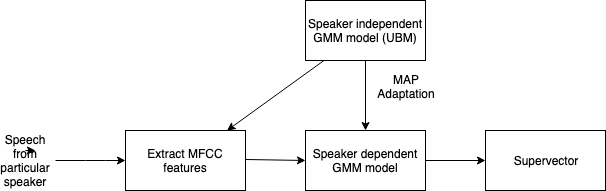
\includegraphics[width=15cm]{figures/supervector.png}
			\centering
			\caption{GMM adaptation.}
			\label{fig:fig-supervector}
		\end{figure}

		\subsubsection{I-vectors}
		I-vectors were introduced in \cite{5545402} as a reduced dimension representation of the GMM supervector using joint factor analysis \cite{kenny2005joint}.
		
		$$ m_s = m_u + Tw_s $$
		
		$m_s$ and $m_u$ are the adapted supervector for a segment $S$ and the UBM supervector, respectively. $w_s$ is the i-vector of the segment $s$. $T$ is the ``total variability matrix" which projects the supervector down to the i-vector representation. $T$ is estimated from the training data using the EM algorithm. I-vectors are generally chosen to be about 400 dimensions.
		
		I-vectors can be compared with simple cosine scoring to judge whether they represent the same speaker or not.
		
		$$ f_{cos}(w_1, w_2) = \frac{w_1.w_2}{|w_1||w_2|} $$
		
		\subsubsection{X-vectors}
		X-vectors are detailed in \cite{snyder2018x}. In this technique, a deep neural network (DNN) is trained to discriminate between the speakers in the training data. Each training example consists of a chunk of features (around 3 seconds) and the corresponding speaker label. An embedding called the x-vector is extracted from a designated layer. Thus, the variable-length utterances are mapped to fixed dimensional x-vectors. Unlike i-vector training which is unsupervised, speaker labels are needed for training \cite{stafylakis2019self}.
		
		An example architecture of the DNN is given in Table \ref{table-xvec-dnn}. $T$ is the segment length, $N$ is the number of speakers. There are layers that operate on speech frames, a statistical pooling layer that aggregates over frame-level representations to give segment-level representations, and in the end a softmax layer. First 5 layers work with a TDNN architecture \cite{peddinti2015time}. The x-vectors are extracted from segment6.
		
		\begin{table}[h]
			\centering
			\begin{tabular}{|c|c|c|c|}
				\hline
				Layer & Layer context & Total context & Input x Output \\
				\hline
				frame1 & [t - 2, t + 2] & 5 & 120x512 \\
				frame2 & \{t - 2, t, t + 2\} & 9 & 1536x512 \\
				frame3 & \{t - 3, t, t + 3\} & 15 & 1536x512 \\
				frame4 & \{t\} & 15 & 512x512 \\
				frame5 & \{t\} & 15 & 512x1500 \\
				stats pooling & [0,T) & T & 1500Tx3000 \\
				segment6 & \{0\} & T & 3000x512 \\
				segment7 & \{0\} & T & 512x512 \\
				softmax & \{0\} & T & 512xN \\
				\hline
			\end{tabular}
			\caption{The x-vector DNN architecture.}
			\label{table-xvec-dnn}
		\end{table}
		
	\subsection{Hierarchical Agglomerative Clustering}
		 Hierarchical Agglomerative Clustering (HAC) is the most commonly used clustering algorithm for diarization. It utilizes a bottom up approach in which the clustering is initialized with one cluster for each data point. It aims at reducing the number of clusters by 1 in each iteration by merging two of the most similar clusters. The basic algorithm is as follows.
		
		\begin{verbatim}
			while (num-clusters > min-clusters && merge-cost <= threshold) {
			    if (size-of-new-cluster <= max-cluster-size) {
			        merge two clusters with lowest cost
			    }
			}
		\end{verbatim}

	\subsection{Distance metrics}
		\subsubsection{Probabilistic Linear Discriminant Analysis}
		Probabilistic Linear Discriminant Analysis (PLDA) \cite{ioffe2006probabilistic} \cite{prince2007probabilistic} is the state-of-the-art scoring technique for diarization. It is used to generate similarity scores between each pair of i-vectors or x-vectors in a given recording. PLDA is a probabilistic extension of Linear Discriminant Analysis (LDA). LDA is similar to Principal Component Analysis (PCA) where data can be projected onto a lower dimension. Unlike PCA whose goal is data representation, the goal of LDA is class separability. Just like LDA, PLDA projects the data onto a lower dimension while maximizing discriminative ability by maximizing the ratio of between-class and within-class variance.
		
		PLDA is used to calculate the log-likelihood ratio as follows. $H_1$ is the hypothesis that the speakers of the segments are the same. $H_0$ is the hypothesis that they are different.
		
		$$ f_{cos}(w_1,w_2) =  \log p(w_1, w_2 | H_1) - \log [ p(w_1|H_0)  p(w_2|H_0) ] $$

\section{Evaluation}

	\subsubsection{Diarization Error Rate (DER)}
		This metric is the most popular for evaluating diarization. Basically, it is the total percentage of reference speaker time that is not correctly attributed to a speaker. ``Correctly attributed" relates to the optimal mapping between reference and system speakers. The DER formula is given below.
		
		$$ DER = \frac{FA + MISS + ERROR}{TOTAL} $$
		
		$TOTAL$ is the sum of durations of all reference speaker segments.
		$FA$ or False Alarm, is the system speaker time that is not attributed to a reference speaker. This is when the system misinterprets a non-speech segment as speech.
		$MISS$ is the reference speaker time that is not accounted for by a system speaker. This is when the system misses a speech segment and classifies it as non-speech.
		$ERROR$ is the total system speaker time that is attributed to the wrong speaker. This is when the system incorrectly guesses the identity of a speaker.
		
		It is easy to see that the best possible DER is 0\%. Also if FA is always zero, 100\% is the upper limit for DER. Because of its definition, speakers with more speaking time tend to contribute more to DER than speakers with less speaking time.

\section{Kaldi toolkit}
	\subsection{Introduction}
	The Kaldi speech recognition toolkit \cite{povey2011kaldi} was started in 2009 at John Hopkins University (JHU) with an aim to create a modern, well-engineered general purpose speech toolkit with a permissive license. Other aims of the project were to have a finite-state transducer (FST) based framework and have extensive linear algebra support. The toolkit depends on some external libraries that are freely available - OpenFST, BLAS and LAPACK. The toolkit includes programs written in C++ that wrap these libraries, which are in turn called from bash/python scripts that can be combined to create complete recipes that do a specific job like speech/speaker recognition, diarization etc.
	
	Kaldi includes ready-to-use complete recipes for popular and widely available datasets such as those provided by the Linguistic Data Consortium (LDC). They are available as subdirectories of the \ttvar{egs} directory in Kaldi's root directory.
	
	\begin{verbatim}
	(base) [acq18mh@snarl ~/workspace]$ ls kaldi/egs
	README.txt            casia_hwdb               fisher_swbd
	aidatatang_200zh      chime1                   formosa
	aishell               chime2                   gale_arabic
	aishell2              chime3                   gale_mandarin
	ami                   chime4                   gp
	an4                   chime5                   heroico
	apiai_decode          cifar                    hkust
	aspire                commonvoice              hub4_english
	aurora4               csj                      hub4_spanish
	babel                 dihard2-voxceleb         iam
	babel_multilang       dihard_2018              iban
	bentham               fame                     ifnenit
	bn_music_speech       farsdat                  librispeech
	callhome_diarization  fisher_callhome_spanish  lre
	callhome_egyptian     fisher_english           lre07
	\end{verbatim}
	
	The C++ executables are have specific functionality so that they can be chained together in a typical Unix-like fashion to create complex pipelines. Given in Figure \ref{fig:fig-kaldi} is a simplified diagram of the Kaldi architecture taken from \cite{povey2011kaldi}.
	
	\begin{figure}[t]
		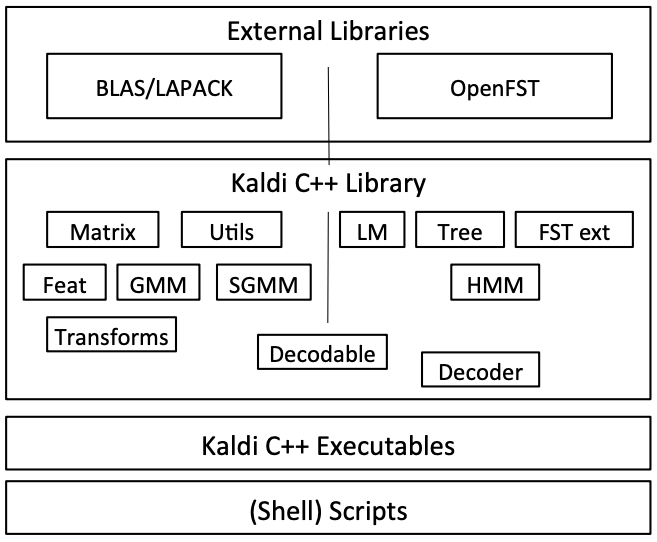
\includegraphics[width=10cm]{figures/kaldi.png}
		\centering
		\caption{Kaldi architecture. Image source \cite{povey2011kaldi}}
		\label{fig:fig-kaldi}
	\end{figure}
	
	\subsection{Briew Overview of a Kaldi Recipe}
	This section describes some important parts of a typical Kaldi recipe. JHU's recipe for the DIHARD 2018 challenge \ttvar{egs/dihard_2018} is used as reference. It looks like the following.
	
	\begin{verbatim}
(base) [acq18mh@snarl kaldi]$ ls -l egs/dihard_2018
-rw-r--r--. acq18mh mini Jun 24 21:43 README.txt
-rwxr-xr-x. acq18mh mini Aug 26 03:26 cmd.sh
drwxr-sr-x. acq18mh mini Aug 19 01:04 conf
drwxr-sr-x. acq18mh mini Sep  7 19:21 data
lrwxrwxrwx. acq18mh mini Jun 24 21:43 diarization ->
 ../../callhome_diarization/v1/diarization
drwxr-sr-x. acq18mh mini Sep  7 19:20 exp
drwxr-sr-x. acq18mh mini Aug 30 01:16 local
drwxr-sr-x. acq18mh mini Sep  7 19:20 mfcc
-rwxr-xr-x. acq18mh mini Jun 24 21:43 path.sh
-rwxr-xr-x. acq18mh mini Aug 26 03:26 run.sh
lrwxrwxrwx. acq18mh mini Jun 24 21:43 sid -> ../../sre08/v1/sid
lrwxrwxrwx. acq18mh mini Jun 24 21:43 steps -> ../../wsj/s5/steps
lrwxrwxrwx. acq18mh mini Jun 24 21:43 utils -> ../../wsj/s5/utils
	\end{verbatim}
	
	Most Kaldi recipes have a top level script called ``run.sh" in the recipe directory. This is the starting point of the recipe. There are several scripts that are reused across many recipes. In many cases this is achieved by creating symlinks to other recipes, as seen by the arrows in the above listing. This recipe reuses scripts from the \ttvar{callhome_diarization}, \ttvar{wsj} and \ttvar{sre08} recipes. Scripts that are specific to this recipe are placed in \ttvar{local}, configuration files are placed in \ttvar{conf} and \ttvar{exp} contains files needed or created during the experiment. The \ttvar{data} directory is important because it holds a lot of information about the data that the experiment works on.
	
	\begin{verbatim}
	(base) [acq18mh@snarl dihard_2018]$ ls -l data
	-rw-r--r--.  1 acq18mh mini 3909183 Aug 28 03:32 feats.scp
	-rw-r--r--.  1 acq18mh mini    1642 Aug 28 03:31 reco2num_spk
	-rw-r--r--.  1 acq18mh mini 1768875 Aug 28 03:31 rttm
	-rw-r--r--.  1 acq18mh mini  808834 Aug 28 03:32 segments
	-rw-r--r--.  1 acq18mh mini  289353 Aug 28 03:32 spk2utt
	drwxr-sr-x. 42 acq18mh mini    4096 Aug 28 03:32 split40
	-rw-r--r--.  1 acq18mh mini  423522 Aug 28 03:32 utt2dur
	-rw-r--r--.  1 acq18mh mini  392200 Aug 28 03:32 utt2num_frames
	-rw-r--r--.  1 acq18mh mini  465297 Aug 28 03:32 utt2spk
	-rw-r--r--.  1 acq18mh mini   27388 Aug 28 03:32 wav.scp
	-rw-r--r--.  1 acq18mh mini   27388 Aug 28 03:32 vad.scp
	\end{verbatim}
	
	There are 3 files that must be created manually in diarization recipes: wav.scp, utt2spk, segments. The wav.scp file holds information about the actual audio files and how to extract a waveform from them in a usable form. The utt2spk file contains identifiers for all utterances mapped to the identity of the speaker who speaks them. The spk2utt file is the opposite and is created automatically. The segments file holds information about the timestamps of the spoken utterances in the audio files. The feats.scp file is created after feature extraction and has the location of the features on disk. The vad.scp file is created after voice activity detection (or SAD) and contains the location of the vectors generated after SAD. These vectors are equal to the MFCCs in length and contain 0's and 1's, classifying each frame as speech or non-speech. The split40 directory contains a split of this ``data directory" into 40 smaller data directories, for parallelization purposes.
